% STATUS: ACTIVE -- 2026-10-26 (user): estimated angle in the local coordinate. States: tracking error (u v w), the two gains, the two
%   local off-diagonal elements a_uw, a_vw of the gain matrix, slopes, and the angles. The angles have no measurement: each step the
%   small angle delta-theta-hat computed from the estimated off-diagonal elements is added to the angle, and all estimates are then
%   expressed in the next local coordinate. H holds only 0 and 1. The error covariance is left open (user).
%   Notation as memory project_notation_unified_2026-10-25 (lambda_c, delta italic; epsilon upright; transpose italic T); EC names
%   e_p, e_a, G_a; local quantities with left superscript v; elements of a local matrix [ . ]_vw.
% Compile: xelatex 1026_local_angle_estimator.tex (from reference/eq17_analysis/derivation/).
\documentclass[11pt,a4paper]{ctexart}
\usepackage[fleqn]{amsmath}
\usepackage{amssymb,bm,upgreek,graphicx}
\setlength{\mathindent}{0pt}
\usepackage{geometry}
\geometry{margin=1.8cm}
\setlength{\parindent}{0pt}
\setlength{\parskip}{0.2em}
\AtBeginDocument{\setlength{\abovedisplayskip}{4pt}\setlength{\belowdisplayskip}{4pt}}
\usepackage{xcolor}
\graphicspath{{figures/}}
\newcommand{\setline}[1]{\par\medskip\noindent{\small\textcolor[gray]{0.35}{#1}}}
\newcommand{\hd}[1]{\par\bigskip\noindent\underline{\textbf{#1}}}
% fonts: upright Greek scalars, bold upright vectors / matrices
\newcommand{\lc}{\lambda_c}
\newcommand{\dl}{\delta}
\newcommand{\bth}{\bm{\uptheta}}
\newcommand{\bep}{\bm{\upvarepsilon}_p}
\newcommand{\Lb}{\bar{\bm{\Lambda}}}
\newcommand{\Sn}{\bm{\Sigma}_n}
\newcommand{\Ab}{\bar{\mathbf A}}
\newcommand{\Ah}{\hat{\mathbf A}}
\newcommand{\Am}{\bar{\mathbf A}_m}
\newcommand{\av}{\bar{\mathbf a}}
\newcommand{\ah}{\hat{\mathbf a}}
\newcommand{\am}{\bar{\mathbf a}_m}
\newcommand{\dpb}{\dl\bar{\mathbf p}}
\newcommand{\dph}{\dl\hat{\mathbf p}}
\newcommand{\Fd}{\bar{\mathbf F}_{dp}}
\newcommand{\Mb}{\mathbf M}
\newcommand{\Mh}{\hat{\mathbf M}}
\newcommand{\I}{\mathbf I}
\newcommand{\V}{\mathbf V}
\newcommand{\Vh}{\hat{\mathbf V}}
\newcommand{\uu}{\mathbf u}
\newcommand{\vv}{\mathbf v}
\newcommand{\ww}{\mathbf w}
\newcommand{\wh}{\hat{\mathbf w}}
\newcommand{\apar}{\bar a_{11}}
\newcommand{\aper}{\bar a_{33}}
\newcommand{\CK}{C_T\,\kappa_T}
\newcommand{\E}{\mathrm{E}}
\newcommand{\T}{T}
\newcommand{\GA}{\begin{bmatrix} F_x & 0 & 0 & F_y & F_z & 0 \\ 0 & F_y & 0 & F_x & 0 & F_z \\ 0 & 0 & F_z & 0 & F_x & F_y \end{bmatrix}}
\newcommand{\Jt}{\dfrac{\partial\bth}{\partial\av}\bigg|_{\Ah}}
\newcommand{\eyl}[1]{\big[\,\mathbf e_p^{\T}[k]\ \ \mathbf e_a^{\T}[k]#1\,\big]^{\T}}
\newcommand{\nv}{\big[\,\mathbf 0\ \ \mathbf 0\ \ -\bep^{\T}[k]\ \ \big(\hat{\mathbf a}'[k]\,\wh^{\T}[k]\,\bep[k]\big)^{\T}\ \ \mathbf 0\ \ \mathbf 0\,\big]^{\T}}
\newcommand{\Jw}{\dfrac{\partial\ww}{\partial\bth}\bigg|_{\hat\bth}}
\newcommand{\vA}{{}^{v}\bar{\mathbf A}}
\newcommand{\vAh}{{}^{v}\hat{\mathbf A}}
\newcommand{\vAm}{{}^{v}\bar{\mathbf A}_m}
\newcommand{\vdp}{{}^{v}\dl\bar{\mathbf p}}
\newcommand{\vdph}{{}^{v}\dl\hat{\mathbf p}}
\newcommand{\vF}{{}^{v}\bar{\mathbf F}_{dp}}
\newcommand{\vM}{{}^{v}\mathbf M}
\newcommand{\vMh}{{}^{v}\hat{\mathbf M}}
\newcommand{\vep}{{}^{v}\bm{\upvarepsilon}_p}
\newcommand{\dd}{\big(\apar - \aper\big)}
\newcommand{\ddh}{\big(\hat a_{11} - \hat a_{33}\big)}
\newcommand{\dth}{\delta\hat\theta}
\newcommand{\ef}{\big[\,\mathbf e_p^{\T}[k]\ \ \mathbf e_a^{\T}[k]\,\big]^{\T}}
\pagestyle{plain}

\begin{document}

\begin{center}\textbf{\large Estimated angle in the local coordinate}\\[2pt]
\small 2026-10-28 \quad local coordinate of the estimate $(u, v, w)$; measurement coordinate $(x, y, z)$\end{center}

%======================================================================
\section{Gain matrix in the local coordinate of the estimate}
\begin{align*}
{}^{V[k]}\hat{\mathbf A}[k] &= \Vh^{\T}[k]\,\hat{\mathbf A}[k]\,\Vh[k] \approx \mathrm{diag}\big(\hat a_{11}[k],\ \hat a_{22}[k],\ \hat a_{33}[k]\big) \\[4pt]
{}^{V[k]}\Ab[k+1] &= \Vh^{\T}[k]\,\Ab[k+1]\,\Vh[k] \\
&\approx \Vh^{\T}[k]\,\Vh[k+1]\;\mathrm{diag}\big(\hat a_{11}[k+1],\ \hat a_{22}[k+1],\ \hat a_{33}[k+1]\big)\;\Vh^{\T}[k+1]\,\Vh[k] \\[4pt]
\Vh^{\T}[k]\,\Vh[k+1] &= \mathbf R_x^{\T}(\hat\theta_x[k])\,\mathbf R_y^{\T}(\hat\theta_y[k])\,\mathbf R_y\big(\hat\theta_y[k] + \dth_y[k]\big)\,\mathbf R_x\big(\hat\theta_x[k] + \dth_x[k]\big) \\
&= \mathbf R_x^{\T}(\hat\theta_x[k])\,\mathbf R_y(\dth_y[k])\,\mathbf R_x(\hat\theta_x[k])\,\mathbf R_x(\dth_x[k])
\end{align*}
\setline{small angle}
\begin{align*}
\mathbf R_y(\dth_y) &\approx \begin{bmatrix} 1 & 0 & \dth_y \\ 0 & 1 & 0 \\ -\dth_y & 0 & 1 \end{bmatrix}, \qquad
\mathbf R_x(\dth_x) \approx \begin{bmatrix} 1 & 0 & 0 \\ 0 & 1 & -\dth_x \\ 0 & \dth_x & 1 \end{bmatrix}
\end{align*}
\setline{product of two small angles left out}
\begin{align*}
\Vh^{\T}[k]\,\Vh[k+1] &\approx \begin{bmatrix}
1 & \sin\hat\theta_x[k]\,\dth_y[k] & \cos\hat\theta_x[k]\,\dth_y[k] \\
-\sin\hat\theta_x[k]\,\dth_y[k] & 1 & -\dth_x[k] \\
-\cos\hat\theta_x[k]\,\dth_y[k] & \dth_x[k] & 1
\end{bmatrix} \\[4pt]
{}^{V[k]}\Ab[k+1] &\approx \begin{bmatrix}
\hat a_{11}[k+1] & 0 & -\big(\hat a_{11}[k] - \hat a_{33}[k]\big)\cos\hat\theta_x[k]\,\dth_y[k] \\
0 & \hat a_{22}[k+1] & \big(\hat a_{22}[k] - \hat a_{33}[k]\big)\,\dth_x[k] \\
\begin{array}{c} -\big(\hat a_{11}[k] - \hat a_{33}[k]\big) \\ \times\cos\hat\theta_x[k]\,\dth_y[k] \end{array} & \begin{array}{c} \big(\hat a_{22}[k] - \hat a_{33}[k]\big) \\ \times\,\dth_x[k] \end{array} & \hat a_{33}[k+1]
\end{bmatrix} \\
&= \begin{bmatrix} \hat a_{11}[k+1] & 0 & \hat a_{13}[k+1] \\ 0 & \hat a_{22}[k+1] & \hat a_{23}[k+1] \\ \hat a_{13}[k+1] & \hat a_{23}[k+1] & \hat a_{33}[k+1] \end{bmatrix}
\end{align*}

%======================================================================
\clearpage
\section{Process in the local coordinate}
\setline{left superscript $v$: local coordinate of $\Vh$; as Section 1 with $\bth - \hat\bth$ in place of $\dth$}
\begin{align*}
\vA &= \Vh^{\T}\,\Ab\,\Vh = \begin{bmatrix} \apar & 0 & \bar a_{13} \\ 0 & \apar & \bar a_{23} \\ \bar a_{13} & \bar a_{23} & \aper \end{bmatrix} \\
\bar a_{23} &= \dd\big(\theta_x - \hat\theta_x\big) \\
\bar a_{13} &= -\dd\cos\hat\theta_x\,\big(\theta_y - \hat\theta_y\big)
\end{align*}
\setline{motion control law}
\begin{align*}
{}^{v}\bar{\mathbf f}_d[k] &= \vAh^{-1}[k]\,\Big\{{}^{v}\bar{\mathbf p}_d[k+1] - {}^{v}\hat{\mathbf p}[k] - \lc\,\big({}^{v}\bar{\mathbf p}_d[k] - {}^{v}\hat{\mathbf p}[k]\big)\Big\}
\end{align*}
\setline{dynamics of tracking error; $F_u, F_v, F_w$: elements of $\vF[k]$}
\begin{align*}
\vdp[k+1] &= \lc\,\vdp[k] - \big(\vA - \vAh[k]\big)\,\vF[k] - \vep[k] \\
\big(\vA - \vAh\big)\,\vF &= \mathbf G_a[k]\,\big[\,\apar - \hat a_{11}\ \ \aper - \hat a_{33}\ \ \bar a_{13} - \hat a_{13}\ \ \bar a_{23} - \hat a_{23}\,\big]^{\T} \\
\mathbf G_a[k] &= \begin{bmatrix} F_u & 0 & F_w & 0 \\ F_v & 0 & 0 & F_w \\ 0 & F_w & F_u & F_v \end{bmatrix}
\end{align*}
\setline{motion along the surface normal; ${}^{v}\ww$: true normal in the local coordinate of the estimate (third column of $\Vh^{\T}\V$, small-angle form of the matrix above with $\bth - \hat\bth$)}
\begin{align*}
\vM[k] &= {}^{v}\Delta\bar{\mathbf p}_d[k] + (1-\lc)\,\vdp_3[k] \\
{}^{v}\ww &= \big[\,\cos\hat\theta_x\,(\theta_y - \hat\theta_y)\ \ \ -(\theta_x - \hat\theta_x)\ \ \ 1\,\big]^{\T}
\end{align*}
\setline{true state}
\begin{align*}
\vdp_1[k+1] &= \vdp_2[k] \\
\vdp_2[k+1] &= \vdp_3[k] \\
\vdp_3[k+1] &= \lc\,\vdp_3[k] - \big(\vA - \vAh[k]\big)\,\vF[k] - \vep[k] \\
\apar[k+1] &= \apar[k] + \apar'[k]\;{}^{v}\ww^{\T}\Big(\vM[k] + \big(\vA - \vAh[k]\big)\,\vF[k] + \vep[k]\Big) \\
\aper[k+1] &= \aper[k] + \aper'[k]\;{}^{v}\ww^{\T}\Big(\vM[k] + \big(\vA - \vAh[k]\big)\,\vF[k] + \vep[k]\Big) \\
\apar'[k+1] &= \apar'[k] \\
\aper'[k+1] &= \aper'[k] \\
\bar a_{13}[k+1] &= \bar a_{13}[k] \\
\bar a_{23}[k+1] &= \bar a_{23}[k] \\
\bth[k+1] &= \bth[k]
\end{align*}

%======================================================================
\clearpage
\section{Estimator}
\begin{align*}
&\big[\,\vdp_1^{\T}\ \ \vdp_2^{\T}\ \ \vdp_3^{\T}\ \ \apar\ \ \aper\ \ \apar'\ \ \aper'\ \ \bar a_{13}\ \ \bar a_{23}\ \ \theta_x\ \ \theta_y\,\big]^{\T} \qquad (17 \times 1,\ d = 2)
\end{align*}
\setline{process outputs in the local coordinate}
\begin{align*}
{}^{v}\dpb_m[k] &= \Vh^{\T}[k]\,\dpb_m[k], \qquad \vAm[k] = \Vh^{\T}[k]\,\Am[k]\,\Vh[k] \\
\bar a_{m,11} &= \tfrac{1}{2}\Big(\big[\vAm\big]_{11} + \big[\vAm\big]_{22}\Big), \qquad \bar a_{m,33} = \big[\vAm\big]_{33}, \qquad
\bar a_{m,13} = \big[\vAm\big]_{13}, \qquad \bar a_{m,23} = \big[\vAm\big]_{23}
\end{align*}
\setline{process outputs, their estimates and the output matrix (no measurement of the angles)}
\begin{align*}
\mathbf y_m[k] &= \begin{bmatrix} {}^{v}\dpb_m[k] \\ \bar a_{m,11}[k] \\ \bar a_{m,33}[k] \\ \bar a_{m,13}[k] \\ \bar a_{m,23}[k] \end{bmatrix}, \qquad
\hat{\mathbf y}[k] = \begin{bmatrix} \vdph_1[k] \\ \hat a_{11}[k] \\ \hat a_{33}[k] \\ \hat a_{13}[k] \\ \hat a_{23}[k] \end{bmatrix}, \qquad
\mathbf H = \begin{bmatrix} \I_3 & \mathbf 0 & \mathbf 0 & \mathbf 0 & \mathbf 0 & \mathbf 0 & \mathbf 0 \\ \mathbf 0 & \mathbf 0 & \mathbf 0 & \I_2 & \mathbf 0 & \mathbf 0 & \mathbf 0 \\ \mathbf 0 & \mathbf 0 & \mathbf 0 & \mathbf 0 & \mathbf 0 & \I_2 & \mathbf 0 \end{bmatrix}
\end{align*}
\setline{feedback: measured $-$ estimate ($\mathbf e_a$: the four gain elements)}
\begin{align*}
\mathbf e_p[k] &= {}^{v}\dpb_m[k] - \vdph_1[k] \\
\mathbf e_a[k] &= \big[\,\bar a_{m,11} - \hat a_{11}\ \ \ \bar a_{m,33} - \hat a_{33}\ \ \ \bar a_{m,13} - \hat a_{13}\ \ \ \bar a_{m,23} - \hat a_{23}\,\big]^{\T}
\end{align*}
\setline{estimator}
\begin{align*}
\vMh[k] &= {}^{v}\Delta\bar{\mathbf p}_d[k] + (1-\lc)\,\vdph_3[k] \\
\vdph_1[k+1] &= \vdph_2[k] + \mathbf L_1[k]\ef \\
\vdph_2[k+1] &= \vdph_3[k] + \mathbf L_2[k]\ef \\
\vdph_3[k+1] &= \lc\,\vdph_3[k] + \mathbf L_3[k]\ef \\
\hat a_{11}[k+1] &= \hat a_{11}[k] + \hat a'_{11}[k]\,\big[\vMh[k]\big]_w + \mathbf L_4[k]\ef \\
\hat a_{33}[k+1] &= \hat a_{33}[k] + \hat a'_{33}[k]\,\big[\vMh[k]\big]_w + \mathbf L_5[k]\ef \\
\hat a'_{11}[k+1] &= \hat a'_{11}[k] + \mathbf L_6[k]\ef \\
\hat a'_{33}[k+1] &= \hat a'_{33}[k] + \mathbf L_7[k]\ef \\
\hat a_{13}[k+1] &= \hat a_{13}[k] + \mathbf L_8[k]\ef \\
\hat a_{23}[k+1] &= \hat a_{23}[k] + \mathbf L_9[k]\ef \\
\hat\bth[k+1] &= \hat\bth[k] + \dth[k] \\
\dth_x[k] &= \frac{\hat a_{23}[k+1]}{\hat a_{11}[k] - \hat a_{33}[k]} \\
\dth_y[k] &= -\frac{\hat a_{13}[k+1]}{\big(\hat a_{11}[k] - \hat a_{33}[k]\big)\cos\hat\theta_x[k]}
\end{align*}
\setline{local coordinate of $\Vh[k+1]$; $\Vh^{\T}[k]\,\Vh[k+1]$ of Section 1}
\begin{align*}
\vdph_i &\leftarrow \big(\Vh^{\T}[k]\,\Vh[k+1]\big)^{\T}\,\vdph_i \\
{}^{V[k+1]}\hat{\mathbf A}[k+1] &\approx \mathrm{diag}\big(\hat a_{11}[k+1],\ \hat a_{22}[k+1],\ \hat a_{33}[k+1]\big), \qquad \hat a_{13}[k+1] \leftarrow 0, \qquad \hat a_{23}[k+1] \leftarrow 0
\end{align*}

%======================================================================
\clearpage
\section{Dynamics of estimation errors}
\setline{estimation error: true $-$ estimate}
\begin{align*}
\mathbf e[k] &= \big[\,\big(\vdp_1 - \vdph_1\big)^{\T}\ \ \big(\vdp_2 - \vdph_2\big)^{\T}\ \ \big(\vdp_3 - \vdph_3\big)^{\T} \\
&\qquad\ \ \apar - \hat a_{11}\ \ \aper - \hat a_{33}\ \ \apar' - \hat a'_{11}\ \ \aper' - \hat a'_{33} \\
&\qquad\ \ \bar a_{13} - \hat a_{13}\ \ \bar a_{23} - \hat a_{23}\ \ \big(\bth - \hat\bth\big)^{\T}\,\big]^{\T}
\end{align*}
\setline{angle: first order; $\bar a_{23}[k+1]$, $\bar a_{13}[k+1]$ in the local coordinate of $\Vh[k]$: $\bar a_{23} = \dd(\theta_x - \hat\theta_x[k])$, $\bar a_{13} = -\dd\cos\hat\theta_x(\theta_y - \hat\theta_y[k])$}
\begin{align*}
\theta_x - \hat\theta_x[k+1] &= \big(\theta_x - \hat\theta_x[k]\big) - \frac{\hat a_{23}[k+1]}{\hat a_{11}[k] - \hat a_{33}[k]} = \frac{\bar a_{23}[k+1] - \hat a_{23}[k+1]}{\hat a_{11}[k] - \hat a_{33}[k]} \\
\theta_y - \hat\theta_y[k+1] &= \big(\theta_y - \hat\theta_y[k]\big) + \frac{\hat a_{13}[k+1]}{\big(\hat a_{11}[k] - \hat a_{33}[k]\big)\cos\hat\theta_x[k]} = -\frac{\bar a_{13}[k+1] - \hat a_{13}[k+1]}{\big(\hat a_{11}[k] - \hat a_{33}[k]\big)\cos\hat\theta_x[k]}
\end{align*}
\setline{other states: first order, feedback terms left out; all elements at step $k$}
\begin{align*}
\vdp_3[k+1] - \vdph_3[k+1] &= \lc\,\big(\vdp_3 - \vdph_3\big) - \mathbf G_a\big[\,\apar - \hat a_{11}\ \ \aper - \hat a_{33}\ \ \bar a_{13} - \hat a_{13}\ \ \bar a_{23} - \hat a_{23}\,\big]^{\T} - \vep \\
\apar[k+1] - \hat a_{11}[k+1] &= \big(\apar - \hat a_{11}\big) + \big(\apar' - \hat a'_{11}\big)\big[\vMh\big]_w
+ \hat a'_{11}(1-\lc)\big[\vdp_3 - \vdph_3\big]_w \\
&\quad + \hat a'_{11}\Big[\mathbf G_a\big[\,\apar - \hat a_{11}\ \ \aper - \hat a_{33}\ \ \bar a_{13} - \hat a_{13}\ \ \bar a_{23} - \hat a_{23}\,\big]^{\T}\Big]_w + \hat a'_{11}\big[\vep\big]_w \\
&\quad + \hat a'_{11}\Big(\cos\hat\theta_x\,\big[\vMh\big]_u\,\big(\theta_y - \hat\theta_y\big) - \big[\vMh\big]_v\,\big(\theta_x - \hat\theta_x\big)\Big) \\
\aper[k+1] - \hat a_{33}[k+1] &= \big(\aper - \hat a_{33}\big) + \big(\aper' - \hat a'_{33}\big)\big[\vMh\big]_w
+ \hat a'_{33}(1-\lc)\big[\vdp_3 - \vdph_3\big]_w \\
&\quad + \hat a'_{33}\Big[\mathbf G_a\big[\,\apar - \hat a_{11}\ \ \aper - \hat a_{33}\ \ \bar a_{13} - \hat a_{13}\ \ \bar a_{23} - \hat a_{23}\,\big]^{\T}\Big]_w + \hat a'_{33}\big[\vep\big]_w \\
&\quad + \hat a'_{33}\Big(\cos\hat\theta_x\,\big[\vMh\big]_u\,\big(\theta_y - \hat\theta_y\big) - \big[\vMh\big]_v\,\big(\theta_x - \hat\theta_x\big)\Big) \\
\bar a_{13}[k+1] - \hat a_{13}[k+1] &= \bar a_{13} - \hat a_{13} \\
\bar a_{23}[k+1] - \hat a_{23}[k+1] &= \bar a_{23} - \hat a_{23}
\end{align*}
\setline{process noise}
\begin{align*}
\mathbf e[k+1] &= \mathbf F_e[k]\,\mathbf e[k] + \big[\,\mathbf 0\ \ \mathbf 0\ \ -\vep^{\T}\ \ \hat a'_{11}[\vep]_w\ \ \hat a'_{33}[\vep]_w\ \ 0\ \ 0\ \ 0\ \ 0\ \ 0\ \ 0\,\big]^{\T} \\
\mathbf Q[k] &= \E\big[\,(\cdot)(\cdot)^{\T}\,\big] + \mathrm{diag}\big(\mathbf 0,\ \mathbf 0,\ \mathbf 0,\ 0,\ 0,\ \mathbf Q_{a'}[k],\ 0,\ 0,\ 0,\ 0\big)
\end{align*}
\setline{estimator feedback matrix and error covariance: left open}

%======================================================================
\clearpage
\section{Simulation at a fixed point}
\setline{wall $\theta_y = 20^\circ$, $\theta_x = 0$; probe held at 15 \textmu m (left) and 5 \textmu m (right); $\hat\bth[0] = \mathbf 0$; 15 \textmu m: 3 seeds with the smallest angle error of seeds 1--10, 5 \textmu m: seeds 1--3; best seed dark}
\begin{center}
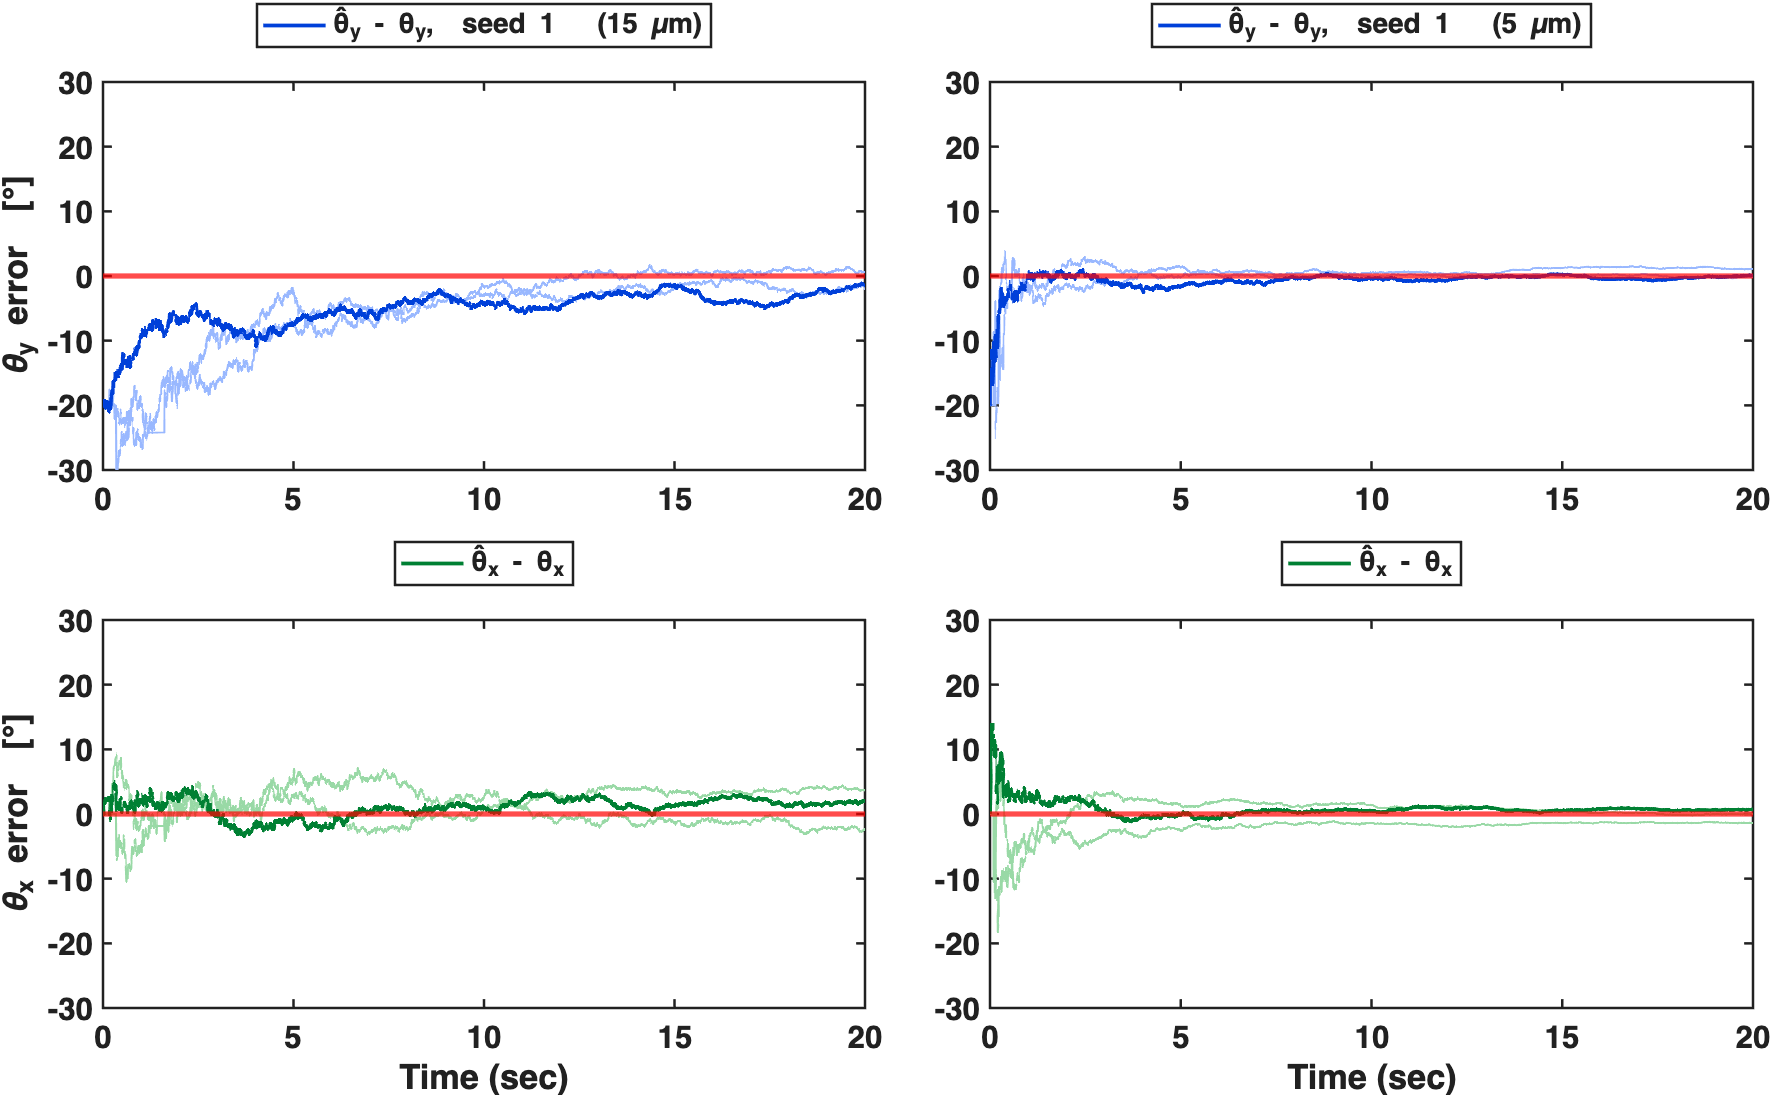
\includegraphics[width=\textwidth]{fig_1026_fixed.png}
\end{center}

\setline{15 and 5\,\textmu m, seed 1; $\hat\bth = \hat\bth[0] + \sum \dth$}
\begin{center}
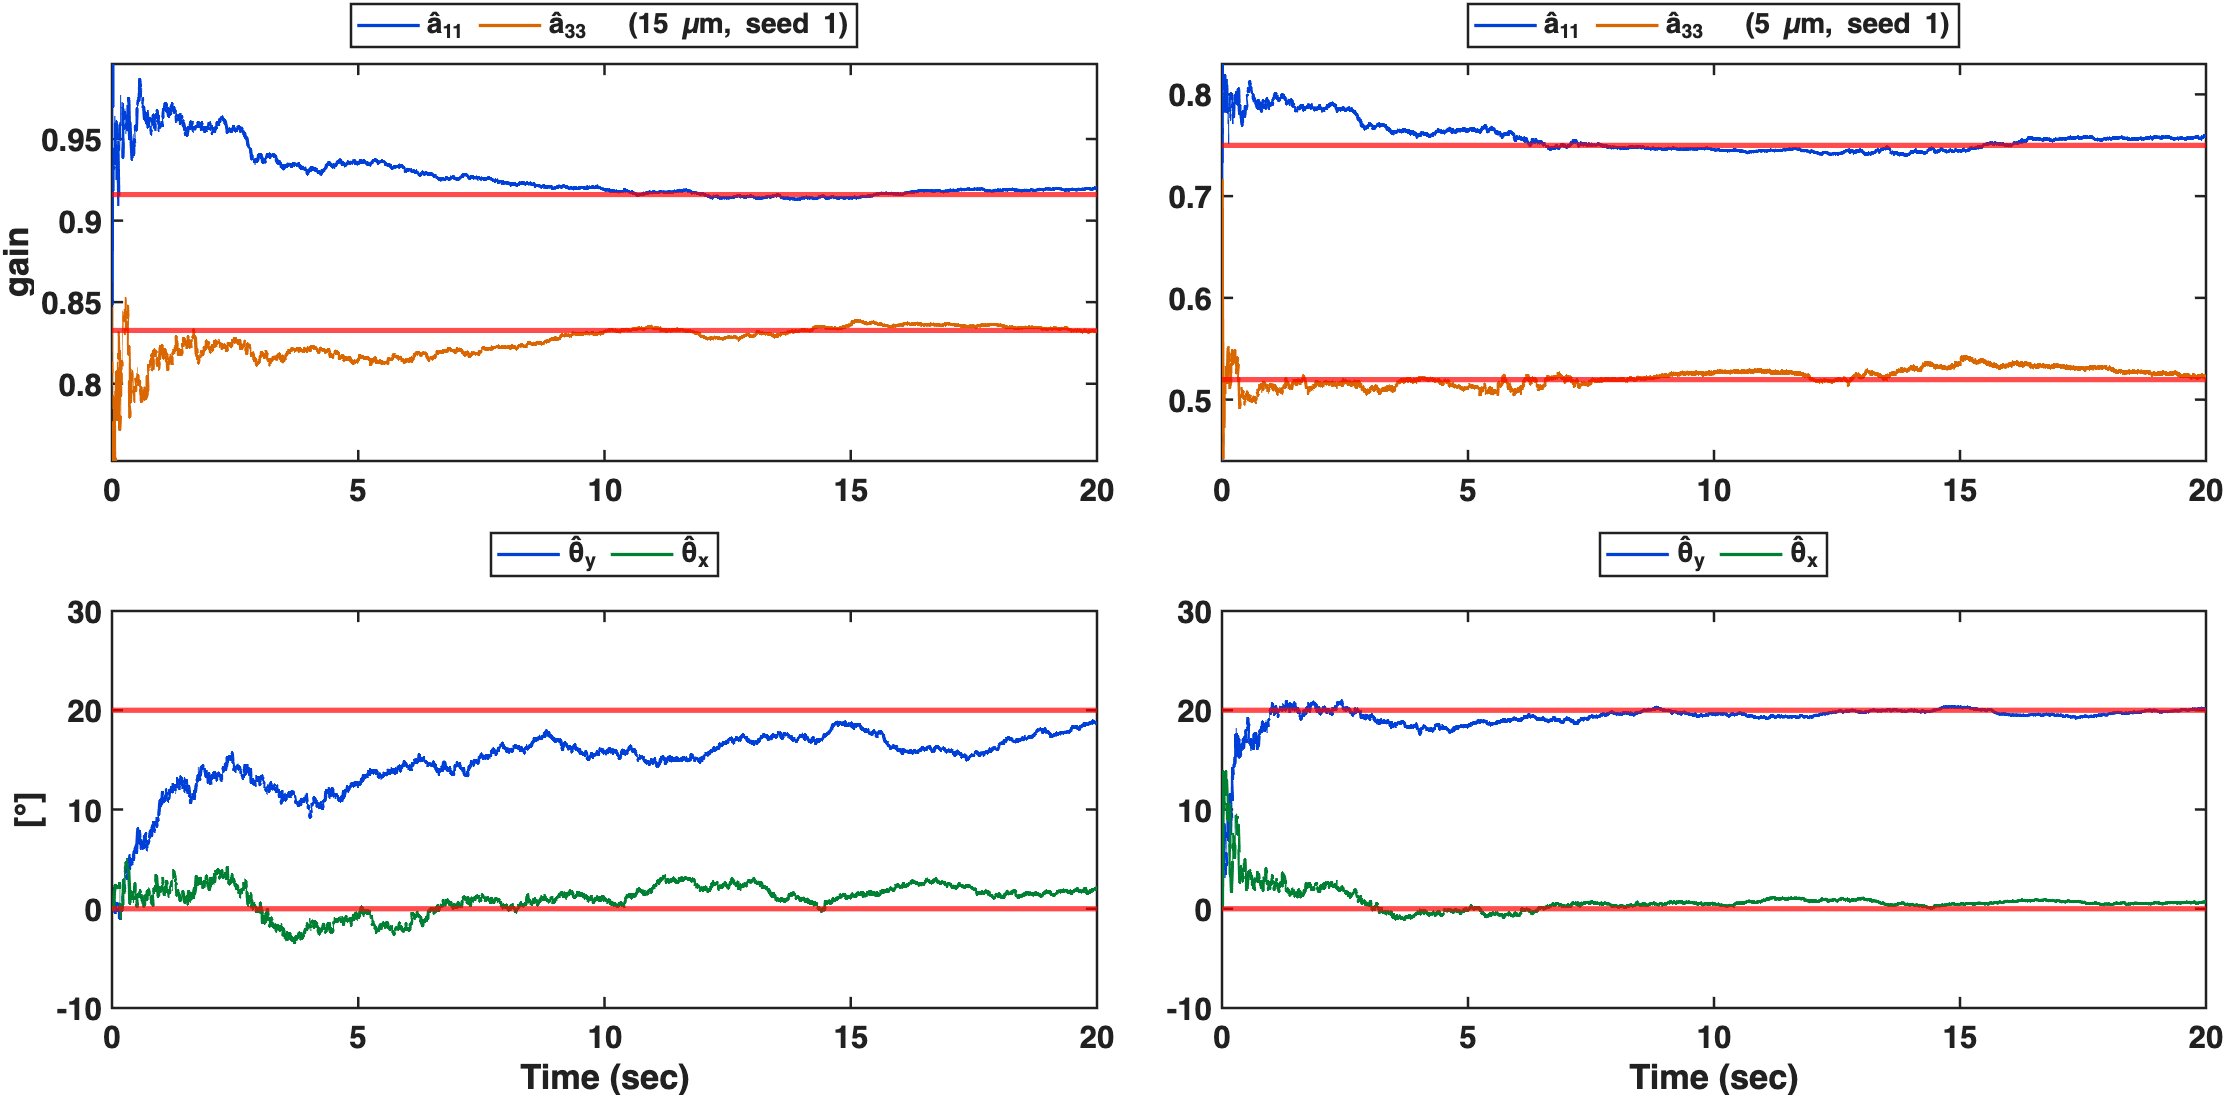
\includegraphics[width=\textwidth]{fig_1026_gain_angle.png}
\end{center}

\end{document}
